%%%%%%%%%%%%%%%%%%%%%%%%%%%%%%%%%%%%%%%%%%%%%%%%%%%%%%%%%%%
\section{Модуль суммы векторов. 4 случая}
%%%%%%%%%%%%%%%%%%%%%%%%%%%%%%%%%%%%%%%%%%%%%%%%%%%%%%%%%%%
Нахождение модуля (длины) вектора, как правило, начинается с \textbf{построения самого вектора}.
Вектор, чей модуль надо найти, в буквальном смысле нужно увидеть, и
только потом из геометрических соображений искать его длину.

Например, чтобы найти модуль суммы векторов,
надо \textbf{сначала построить} сумму векторов и только
\textbf{потом искать} её модуль.
%%%%%%%%%%%%%%%%%%%%%%%%%%%%%%%%%%%%%%%%%%%%%%%%%%%%%%%%%%%
\subsection{Векторы сонаправлены}
%%%%%%%%%%%%%%%%%%%%%%%%%%%%%%%%%%%%%%%%%%%%%%%%%%%%%%%%%%%
Пусть $\vv{a}$ и $\vv{b}$ \bdash сонаправленные векторы. Сложим их по правилу треугольника.
Для этого совместим начало вектора $\vv{b}$ и конец вектора $\vv{a}$. Вектор $\vv{c}$,
проведённый из начала $\vv{a}$ в конец $\vv{b}$, является их суммой.

\begin{figure}[h!]
  \centering
  \begin{tikzpicture}[thick]
    \coordinate (A) at (1cm,0cm);
    \coordinate (B) at (5cm,0cm);
    \coordinate (C) at (6cm,0cm);
    \coordinate (D) at (8cm,0cm);
    
    \draw [blue, -Latex, very thick] (A) -- node[above,black] {\large $\vv{a}$}(B);
    \draw [blue, -Latex, very thick] (C) -- node[above,black] {\large $\vv{b}$}(D);
    
  \end{tikzpicture}\hspace{1.4cm}
  \begin{tikzpicture}[thick]
    \coordinate (A) at (1cm,0cm);
    \coordinate (B) at (5cm,0cm);
    \coordinate (C) at (5cm,0cm);
    \coordinate (D) at (7cm,0cm);
    \coordinate (E) at (1cm,-0.5cm);
    \coordinate (F) at (7cm,-0.5cm);
    
    \draw [blue, -Latex, very thick] (A) -- node[above,black] {\large $\vv{a}$}(B);
    \draw [blue, -Latex, very thick] (C) -- node[above,black] {\large $\vv{b}$}(D);
    \draw [red, -Latex, very thick] (E) -- (F);
    
    \draw (4.2cm,-1cm) node {\large $\vv{c} =\vv{a}+\vv{b}$};
  \end{tikzpicture}
  \caption{\small Сложение сонаправленных векторов.}\label{pic:sum1}
\end{figure}

Как видно из рисунка, модуль суммы сонаправленных векторов равен сумме их модулей:
{\large
  \begin{align}
    \hly{c = a + b.}
  \end{align}
}

\clearpage

%%%%%%%%%%%%%%%%%%%%%%%%%%%%%%%%%%%%%%%%%%%%%%%%%%%%%%%%%%%
\subsection{Векторы противоположно направлены}
%%%%%%%%%%%%%%%%%%%%%%%%%%%%%%%%%%%%%%%%%%%%%%%%%%%%%%%%%%%
Пусть $\vv{a}$ и $\vv{b}$ \bdash противоположно направленные векторы.
Сложим их также по правилу треугольника.
Для этого совместим начало вектора $\vv{b}$ и конец вектора $\vv{a}$. Вектор $\vv{c}$,
проведённый из начала $\vv{a}$ в конец $\vv{b}$, является их суммой.

\begin{figure}[h!]
  \centering
  \begin{tikzpicture}[thick]
    \coordinate (A) at (1cm,0cm);
    \coordinate (B) at (5cm,0cm);
    \coordinate (C) at (6cm,0cm);
    \coordinate (D) at (8cm,0cm);
    
    \draw [blue, -Latex, very thick] (A) -- node[above,black] {\large $\vv{a}$}(B);
    \draw [blue, -Latex, very thick] (D) -- node[above,black] {\large $\vv{b}$}(C);
    
  \end{tikzpicture}\hspace{1.4cm}
  \begin{tikzpicture}[thick]
    \coordinate (A) at (1cm,0cm);
    \coordinate (B) at (5cm,0cm);
    \coordinate (C) at (5cm,0cm);
    \coordinate (D) at (3cm,0cm);
    \coordinate (E) at (1cm,-0.5cm);
    \coordinate (F) at (3cm,-0.5cm);
    
    \draw [blue, -Latex, very thick] (A) -- (B);
    \draw [blue, -Latex, very thick] (B) -- (D);
    \draw [red, -Latex, very thick] (E) -- (F);
    
    \draw (4.8cm,0.6cm) node {\large $\vv{a}$};
    \draw (3.2cm,0.6cm) node {\large $\vv{b}$};
    \draw (2.4cm,-1cm) node {\large $\vv{c} =\vv{a}+\vv{b}$};
  \end{tikzpicture}
  \caption{\small Сложение противоположно направленных векторов.}\label{pic:sum2}
\end{figure}

Как видно из рисунка, модуль суммы противоположно направленных векторов
равен разности их модулей:
{\large
  \begin{align}
    \hly{c = a - b.}
  \end{align}
}
%%%%%%%%%%%%%%%%%%%%%%%%%%%%%%%%%%%%%%%%%%%%%%%%%%%%%%%%%%%
\subsection{Векторы перпендикулярны}
%%%%%%%%%%%%%%%%%%%%%%%%%%%%%%%%%%%%%%%%%%%%%%%%%%%%%%%%%%%
Сложим перпендикулярные векторы $\vv{a}$ и $\vv{b}$ по правилу треугольника.
Для этого совместим начало вектора $\vv{b}$ и конец вектора $\vv{a}$. Вектор $\vv{c}$,
проведённый из начала $\vv{a}$ в конец $\vv{b}$, является их суммой.

\begin{figure}[h!]
  \centering
  \begin{tikzpicture}[thick]
    \coordinate (A) at (1cm,0cm);
    \coordinate (B) at (1cm,3cm);
    \coordinate (C) at (3cm,0cm);
    \coordinate (D) at (5cm,0cm);
    \coordinate (E) at (-0.5cm,0cm);
    \coordinate (F) at (6cm,0cm);
        
    \draw [blue, -Latex, very thick] (A) -- node[left,black] {\large $\vv{a}$}(B);
    \draw [blue, -Latex, very thick] (C) -- node[above,black] {\large $\vv{b}$}(D);
    \draw [dashed] (E) -- (C);
    \draw [dashed] (D) -- (F);
    % right angle
    \draw (1,0.3)-|(1.3,0);

  \end{tikzpicture}\hspace{1.7cm}
  \begin{tikzpicture}[thick]
    \coordinate (A) at (1cm,0cm);
    \coordinate (B) at (1cm,3cm);
    \coordinate (C) at (3cm,3cm);
    
    \draw [blue, -Latex, very thick] (A) -- node[left,black] {\large $\vv{a}$} (B);
    \draw [blue, -Latex, very thick] (B) -- node[above,black] {\large $\vv{b}$}(C);
    \draw [red, -Latex, very thick] (A) -- (C);
    % right angle
    \draw (1,2.7)-|(1.3,3);
    
    \draw (3.6cm,1.6cm) node {\large $\vv{c} =\vv{a}+\vv{b}$};
  \end{tikzpicture}
  \caption{\small Сложение перпендикулярных векторов.}\label{pic:sum3}
\end{figure}

Векторы $\vv{a}$, $\vv{b}$ и $\vv{c}$ образуют прямоугольный треугольник,
в котором катеты равны $a$ и $b$, а гипотенуза \bdash $c$.
Тогда модуль суммы найдём \textbf{по теореме Пифагора}:
{\large
  \begin{align}
    \hly{c = \sqrt{a^2 + b^2}.}
  \end{align}
}
%%%%%%%%%%%%%%%%%%%%%%%%%%%%%%%%%%%%%%%%%%%%%%%%%%%%%%%%%%%
\subsection{Векторы направлены под произвольным углом}
%%%%%%%%%%%%%%%%%%%%%%%%%%%%%%%%%%%%%%%%%%%%%%%%%%%%%%%%%%%
Перед тем как говорить о нахождении модуля суммы векторов,
направленных под произвольным углом, уточним понятие
\textbf{угла между векторами}. 

Приведём произвольные векторы $\vv{a}$ и $\vv{b}$ к общему началу.
В качестве угла между векторами можно взять любой из двух указанных
на рисунке~\ref{pic:vec_ugol} углов $\upalpha_1$ и $\upalpha_2$.
Из двух углов $\upalpha_1$ и $\upalpha_2$ один не превосходит $\uppi = 180^\circ$.
На рисунке это угол $\upalpha_1$.
В дальнейшем \textbf{углом между векторами} будем называть тот угол, который не превосходит $\uppi$.


Таким образом, если векторы $\vv{a}$ и $\vv{b}$ привести к общему началу, то
углом между ними называется \textbf{наименьший из двух углов}.
\begin{figure}[h]
  \centering
  \begin{tikzpicture}[thick]
    \coordinate (A) at (0cm,0cm);
    \coordinate (B) at (-2cm,3cm);
    \coordinate (C) at (4cm,0cm);
   
    % angles
    \tkzMarkAngle[arc=l, size=0.8cm, mark=none, fill=yellow!30](C,A,B)
    \tkzLabelAngle[pos = 1.2](C,A,B){$\upalpha_1$}
    \tkzMarkAngle[arc=ll, size=0.8cm, mark=none](B,A,C)
    \tkzLabelAngle[pos = 1.2](B,A,C){$\upalpha_2$}
    %\draw (1.1,0.3) node {$\upalpha_2$};

    % vectors
    \draw [blue, -Latex, very thick] (A) -- node[below left,black] {\large $\vv{a}$}(B);
    \draw [blue, -Latex, very thick] (A) -- node[below,black] {\large $\vv{b}$}(C);
    
  \end{tikzpicture}
  \caption{\small Угол между векторами.}\label{pic:vec_ugol}
\end{figure}

\clearpage

%%%%%%%%%%%%%%%%%%%%%%%%%%%%%%%%%%%%%%%%%%%%%%%%%%%%%%%%%%%
\subsubsection{Острый угол между векторами}
%%%%%%%%%%%%%%%%%%%%%%%%%%%%%%%%%%%%%%%%%%%%%%%%%%%%%%%%%%%
Пусть $\vv{a}$ и $\vv{b}$ \bdash два вектора, модули которых известны.
Совместим векторы началами, острый угол между ними известен и равен $\upalpha$.
Найдём модуль суммы этих векторов.

\begin{figure}[h]
  \centering
  \begin{tikzpicture}[thick]
    \coordinate (A) at (0cm,0cm);
    \coordinate (B) at (3cm,3cm);
    \coordinate (C) at (7cm,3cm);
    \coordinate (H) at (4cm,0cm);

    % angle
    %\tkzMarkAngle[arc=l, size=0.8cm, fill=yellow!30](H,A,B)
    \tkzMarkAngle[arc=l, size=0.8cm, mark=none](H,A,B)
    \tkzLabelAngle[pos = 1.2](H,A,B){$\upalpha$}
   
    \draw [blue, -Latex, very thick] (A) -- node[above left,black] {\large $\vv{a}$}(B);
    \draw [blue, -Latex, very thick] (A) -- node[below,black] {\large $\vv{b}$}(H);

  \end{tikzpicture}
  \caption{\small Острый угол между векторами.}\label{pic:sum_ugol1}
\end{figure}

Для этого построим сумму векторов по правилу параллелограмма. В построенном
параллелограмме $ABCD$ на рисунке~\ref{pic:sum_ugol11}
необходимо найти длину диагонали $c = AC$.
Рассмотрим треугольник $ABC$, в котором две стороны $a$ и $b$ известны, а угол
между ними будет равен $(\uppi-\upalpha)$, так как сумма углов в параллелограмме,
прилежащих к одной стороне, равна $\uppi$.
\begin{figure}[h]
  \centering
  \begin{tikzpicture}[thick, scale = 0.8]
    \coordinate[label=below left:$A$] (A) at (0cm,0cm);
    \coordinate[label=above left:$B$] (B) at (3cm,3cm);
    \coordinate[label=above right:$C$] (C) at (7cm,3cm);
    \coordinate[label=below right:$D$] (D) at (4cm,0cm);

    \draw [blue, -Latex, very thick] (A) -- node[above left,black] {\large $\vv{a}$}(B);
    \draw [dashed] (B) -- (C);
    \draw [red, -Latex, very thick] (A) -- (C);
    \draw [blue, -Latex, very thick] (A) --  node[below,black] {\large $\vv{b}$}(D);
    \draw [dashed] (D) -- (C);

    \draw (8.3cm,2.3cm) node {\large $\vv{c} =\vv{a}+\vv{b}$};
  \end{tikzpicture}
  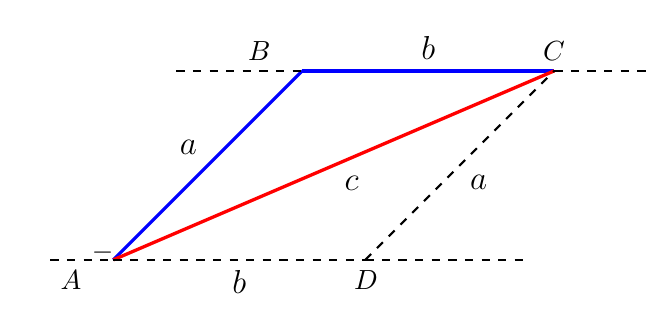
\begin{tikzpicture}[thick, scale = 0.8]
    \coordinate[label=below left:$A$] (A) at (0cm,0cm);
    \coordinate[label=above left:$B$] (B) at (3cm,3cm);
    \coordinate[label=above right:$C$] (C) at (7cm,3cm);
    \coordinate (D) at (-1cm,0cm);
    \coordinate (E) at (6.5cm,0cm);
    \coordinate (F) at (1cm,3cm);
    \coordinate (G) at (8.5cm,3cm);
    \coordinate[label=below right:$D$] (H) at (4cm,0cm);

    \tkzMarkAngle[arc=ll, size=0.6cm, mark=none, fill=yellow!30](A,B,G)
    \tkzLabelAngle[pos = 1](A,B,G){$\uppi-\upalpha$}
    
    \draw [blue, very thick] (A) -- node[above left,black] {\large $a$} (B);
    \draw [blue, very thick] (B) -- node[above, black] {\large $b$} (C);
    \draw [red, very thick] (A) -- node[below right, black] {\large $c$} (C);
    \draw [dashed] (D) -- (A);
    \draw [dashed] (A) -- node[below, black] {\large $b$} (H);
    \draw [dashed] (H) -- (E);
    \draw [dashed] (F) -- (B);
    \draw [dashed] (C) -- (G);
    \draw [dashed] (H) -- node[below right, black] {\large $a$} (C);

    \tkzMarkAngle[arc=l, size=0.8cm, mark=none](E,A,B)
    \tkzLabelAngle[pos = 1.2](E,A,C){$\upalpha$}
  \end{tikzpicture}
  \caption{\small Сумма векторов с острым углом между ними.}\label{pic:sum_ugol11}
\end{figure}

Таким образом в треугольнике $ABC$ известны две стороны и угол между ними.
Третью сторону найдём \textbf{по теореме косинусов}:
\begin{align}
  c = \sqrt{a^2 + b^2 - 2 a b\cos(\uppi-\upalpha)}.
\end{align}
Так как $\cos(\uppi-\upalpha) = -\cos\upalpha$, то окончательно:
{\large
  \begin{align}
    \hly{c = \sqrt{a^2 + b^2 + 2 a b\cos\upalpha}.}
  \end{align}
}

\clearpage

%%%%%%%%%%%%%%%%%%%%%%%%%%%%%%%%%%%%%%%%%%%%%%%%%%%%%%%%%%%
\subsubsection{Тупой угол между векторами}
%%%%%%%%%%%%%%%%%%%%%%%%%%%%%%%%%%%%%%%%%%%%%%%%%%%%%%%%%%%
Аналогично построим сумму векторов с тупым углом между ними и найдём
её модуль.
\begin{figure}[h]
  \centering
  \begin{tikzpicture}[thick]
    \coordinate (A) at (0cm,0cm);
    \coordinate (B) at (-2cm,3cm);
    \coordinate (C) at (2cm,3cm);
    \coordinate (D) at (4cm,0cm);

    % angle
    \tkzMarkAngle[arc=l, size=0.8cm, mark=none](D,A,B)
    \tkzLabelAngle[pos = 1.2](D,A,B){$\upalpha$}
   
    \draw [blue, -Latex, very thick] (A) -- node[below left,black] {\large $\vv{a}$}(B);
    \draw [blue, -Latex, very thick] (A) -- node[below,black] {\large $\vv{b}$}(D);

  \end{tikzpicture}
  \caption{\small Тупой угол между векторами.}\label{pic:sum_ugol2}
\end{figure}

В построенном параллелограмме $ABCD$ на рисунке~\ref{pic:sum_ugol21}
рассмотрим треугольник $ABC$,
в котором известны две стороны $a$, $b$ и угол между ними $(\uppi-\upalpha)$.

\begin{figure}[h]
  \centering
  \begin{tikzpicture}[thick, scale = 0.9]
    \coordinate [label=below left:$A$](A) at (0cm,0cm);
    \coordinate [label=above left:$B$](B) at (-2cm,3cm);
    \coordinate [label=above right:$C$](C) at (2cm,3cm);
    \coordinate [label=below right:$D$](D) at (4cm,0cm);
    
    \draw [blue, -Latex, very thick] (A) -- node[below left,black] {\large $\vv{a}$}(B);
    \draw [dashed] (B) -- (C);
    \draw [red, -Latex, very thick] (A) -- (C);
    \draw [blue, -Latex, very thick] (A) -- node[below,black] {\large $\vv{b}$}(D);
    \draw [dashed] (D) -- (C);
    
    \draw (4.2cm,2.8cm) node {\large $\vv{c} =\vv{a}+\vv{b}$};
  \end{tikzpicture}\hspace{0.5cm}
  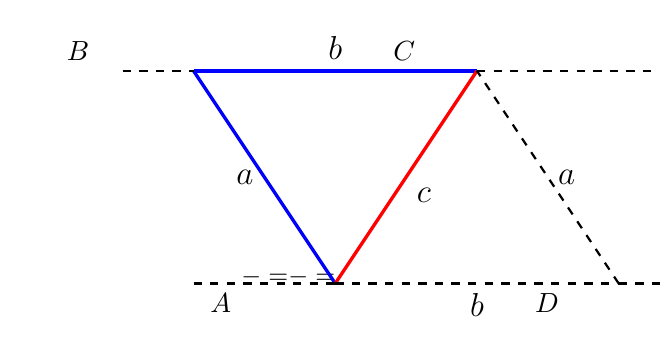
\begin{tikzpicture}[thick, scale = 0.9]
    \coordinate[label=below left:$A$] (A) at (0cm,0cm);
    \coordinate[label=above left:$B$] (B) at (-2cm,3cm);
    \coordinate[label=above right:$C$] (C) at (2cm,3cm);
    \coordinate (D) at (-2cm,0cm);
    \coordinate (E) at (5.5cm,0cm);
    \coordinate (F) at (-3cm,3cm);
    \coordinate (G) at (4.5cm,3cm);
    \coordinate[label=below right:$D$] (H) at (4cm,0cm);
    
    \tkzMarkAngle[arc=ll, size=0.6cm, mark=none, fill=yellow!30](A,B,C)
    \tkzLabelAngle[pos = 0.7, right](A,B,C){\small $\uppi-\upalpha=\upbeta$}
    \tkzMarkAngle[arc=ll, size=0.6cm, mark=none, fill=yellow!30](B,A,D)
    \tkzLabelAngle[pos = 0.7, left](B,A,D){\small $\uppi-\upalpha=\upbeta$}
    
    \draw [blue, very thick] (A) -- node[left,black] {\large $a$} (B);
    \draw [blue, very thick] (B) -- node[above, black] {\large $b$} (C);
    \draw [red, very thick] (A) -- node[below right, black] {\large $c$} (C);
    \draw [dashed] (D) -- (A);
    \draw [dashed] (A) -- node[below, black] {\large $b$} (H);
    \draw [dashed] (H) -- (E);
    \draw [dashed] (F) -- (B);
    \draw [dashed] (C) -- (G);
    \draw [dashed] (H) -- node[right, black] {\large $a$} (C);
    
    \tkzMarkAngle[arc=l, size=0.6cm, mark=none](E,A,B)
    \tkzLabelAngle[pos = 1](C,A,B){$\upalpha$}
  \end{tikzpicture}
  \caption{\small Сумма векторов с тупым углом между ними.}\label{pic:sum_ugol21}
\end{figure}

Так же как в и случае с острым углом третью сторону найдём \textbf{по теореме косинусов}:
\begin{align}
  c = \sqrt{a^2 + b^2 - 2 ab\cos(\uppi-\upalpha)}.
\end{align}

Заметим, что угол $(\uppi-\upalpha)$ является острым (так как $\upalpha$ \bdash тупой),
поэтому уместно переобозначить $(\uppi-\upalpha) = \upbeta$ и применить теорему
косинусов именно для этого угла:
{\large
  \begin{align}
    \hly{c = \sqrt{a^2 + b^2 - 2 a b\cos\upbeta}.}
  \end{align}
}
